\section{eo\-One\-Max\-Mutation$<$ Genotype\-T $>$ Class Template Reference}
\label{classeo_one_max_mutation}\index{eoOneMaxMutation@{eoOneMaxMutation}}
Always write a comment in this format before class definition if you want the class to be documented by Doxygen.  


{\tt \#include $<$eo\-One\-Max\-Mutation.h$>$}

Inheritance diagram for eo\-One\-Max\-Mutation$<$ Genotype\-T $>$::\begin{figure}[H]
\begin{center}
\leavevmode
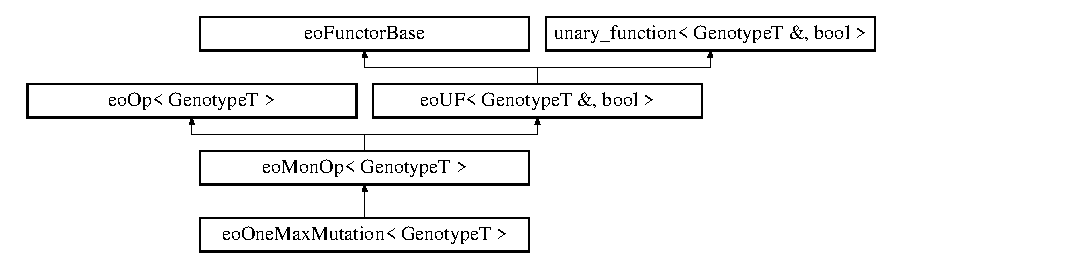
\includegraphics[height=3.15049cm]{classeo_one_max_mutation}
\end{center}
\end{figure}
\subsection*{Public Member Functions}
\begin{CompactItemize}
\item 
{\bf eo\-One\-Max\-Mutation} ()\label{classeo_one_max_mutation_a0}

\begin{CompactList}\small\item\em Ctor - no requirement. \item\end{CompactList}\item 
string {\bf class\-Name} () const \label{classeo_one_max_mutation_a1}

\begin{CompactList}\small\item\em The class name. Used to display statistics. \item\end{CompactList}\item 
bool {\bf operator()} (Genotype\-T \&\_\-genotype)
\begin{CompactList}\small\item\em modifies the parent \item\end{CompactList}\end{CompactItemize}


\subsection{Detailed Description}
\subsubsection*{template$<$class Genotype\-T$>$ class eo\-One\-Max\-Mutation$<$ Genotype\-T $>$}

Always write a comment in this format before class definition if you want the class to be documented by Doxygen. 

THere is NO ASSUMPTION on the class Genoype\-T. In particular, it does not need to derive from {\bf EO}{\rm (p.\,\pageref{class_e_o})} 



Definition at line 25 of file eo\-One\-Max\-Mutation.h.

\subsection{Member Function Documentation}
\index{eoOneMaxMutation@{eo\-One\-Max\-Mutation}!operator()@{operator()}}
\index{operator()@{operator()}!eoOneMaxMutation@{eo\-One\-Max\-Mutation}}
\subsubsection{\setlength{\rightskip}{0pt plus 5cm}template$<$class Genotype\-T$>$ bool {\bf eo\-One\-Max\-Mutation}$<$ Genotype\-T $>$::operator() (Genotype\-T \& {\em \_\-genotype})\hspace{0.3cm}{\tt  [inline, virtual]}}\label{classeo_one_max_mutation_a2}


modifies the parent 

\begin{Desc}
\item[Parameters:]
\begin{description}
\item[{\em \_\-genotype}]The parent genotype (will be modified)\end{description}
\end{Desc}


Requirement if (\_\-genotype has been modified) is\-Modified = true; else is\-Modified = false; 

Implements {\bf eo\-UF$<$ Genotype\-T \&, bool $>$} {\rm (p.\,\pageref{classeo_u_f_a1})}.

Definition at line 47 of file eo\-One\-Max\-Mutation.h.

The documentation for this class was generated from the following file:\begin{CompactItemize}
\item 
eo\-One\-Max\-Mutation.h\end{CompactItemize}
